% Options for packages loaded elsewhere
\PassOptionsToPackage{unicode}{hyperref}
\PassOptionsToPackage{hyphens}{url}
\PassOptionsToPackage{dvipsnames,svgnames,x11names}{xcolor}
%
\documentclass[
]{article}
\usepackage{amsmath,amssymb}
\usepackage{lmodern}
\usepackage{setspace}
\usepackage{iftex}
\ifPDFTeX
  \usepackage[T1]{fontenc}
  \usepackage[utf8]{inputenc}
  \usepackage{textcomp} % provide euro and other symbols
\else % if luatex or xetex
  \usepackage{unicode-math}
  \defaultfontfeatures{Scale=MatchLowercase}
  \defaultfontfeatures[\rmfamily]{Ligatures=TeX,Scale=1}
\fi
% Use upquote if available, for straight quotes in verbatim environments
\IfFileExists{upquote.sty}{\usepackage{upquote}}{}
\IfFileExists{microtype.sty}{% use microtype if available
  \usepackage[]{microtype}
  \UseMicrotypeSet[protrusion]{basicmath} % disable protrusion for tt fonts
}{}
\makeatletter
\@ifundefined{KOMAClassName}{% if non-KOMA class
  \IfFileExists{parskip.sty}{%
    \usepackage{parskip}
  }{% else
    \setlength{\parindent}{0pt}
    \setlength{\parskip}{6pt plus 2pt minus 1pt}}
}{% if KOMA class
  \KOMAoptions{parskip=half}}
\makeatother
\usepackage{xcolor}
\usepackage[margin=1in]{geometry}
\usepackage{graphicx}
\makeatletter
\def\maxwidth{\ifdim\Gin@nat@width>\linewidth\linewidth\else\Gin@nat@width\fi}
\def\maxheight{\ifdim\Gin@nat@height>\textheight\textheight\else\Gin@nat@height\fi}
\makeatother
% Scale images if necessary, so that they will not overflow the page
% margins by default, and it is still possible to overwrite the defaults
% using explicit options in \includegraphics[width, height, ...]{}
\setkeys{Gin}{width=\maxwidth,height=\maxheight,keepaspectratio}
% Set default figure placement to htbp
\makeatletter
\def\fps@figure{htbp}
\makeatother
\setlength{\emergencystretch}{3em} % prevent overfull lines
\providecommand{\tightlist}{%
  \setlength{\itemsep}{0pt}\setlength{\parskip}{0pt}}
\setcounter{secnumdepth}{-\maxdimen} % remove section numbering
\newlength{\cslhangindent}
\setlength{\cslhangindent}{1.5em}
\newlength{\csllabelwidth}
\setlength{\csllabelwidth}{3em}
\newlength{\cslentryspacingunit} % times entry-spacing
\setlength{\cslentryspacingunit}{\parskip}
\newenvironment{CSLReferences}[2] % #1 hanging-ident, #2 entry spacing
 {% don't indent paragraphs
  \setlength{\parindent}{0pt}
  % turn on hanging indent if param 1 is 1
  \ifodd #1
  \let\oldpar\par
  \def\par{\hangindent=\cslhangindent\oldpar}
  \fi
  % set entry spacing
  \setlength{\parskip}{#2\cslentryspacingunit}
 }%
 {}
\usepackage{calc}
\newcommand{\CSLBlock}[1]{#1\hfill\break}
\newcommand{\CSLLeftMargin}[1]{\parbox[t]{\csllabelwidth}{#1}}
\newcommand{\CSLRightInline}[1]{\parbox[t]{\linewidth - \csllabelwidth}{#1}\break}
\newcommand{\CSLIndent}[1]{\hspace{\cslhangindent}#1}
\usepackage{fancyhdr}
\pagestyle{fancy}
\fancyhead[L]{DUTHIE, AB}
\fancyhead[R]{SPARROW BODY LENGTH DECREASES SURVIVAL}
\usepackage{lineno}
\linenumbers
\usepackage[misc]{ifsym}
\ifLuaTeX
  \usepackage{selnolig}  % disable illegal ligatures
\fi
\IfFileExists{bookmark.sty}{\usepackage{bookmark}}{\usepackage{hyperref}}
\IfFileExists{xurl.sty}{\usepackage{xurl}}{} % add URL line breaks if available
\urlstyle{same} % disable monospaced font for URLs
\hypersetup{
  pdftitle={High sparrow body length decreases survival},
  pdfauthor={Brad Duthie},
  colorlinks=true,
  linkcolor={blue},
  filecolor={Maroon},
  citecolor={Blue},
  urlcolor={Blue},
  pdfcreator={LaTeX via pandoc}}

\title{High sparrow body length decreases survival}
\usepackage{etoolbox}
\makeatletter
\providecommand{\subtitle}[1]{% add subtitle to \maketitle
  \apptocmd{\@title}{\par {\large #1 \par}}{}{}
}
\makeatother
\subtitle{A demonstration of Rmarkdown using Herman Bumpus' data}
\author{Brad Duthie}
\date{Biological and Environmental Sciences, University of Stirling,
Stirling, UK, FK9 4LA}

\begin{document}
\maketitle

\setstretch{2}
\hypertarget{abstract}{%
\section{Abstract}\label{abstract}}

Writing documents in Rmarkdown using Rstudio can make scientific
workflow more efficient, and here I demonstrate how a scientific
manuscript can be written using a classical data set first published by
Herman Bumpus. I integrate Bumpus' data with Rmarkdown to produce a
sample manuscript, testing whether or not sparrow body length decreases
survival following a storm in southern New England. Using a t-test, I
show that surviving birds have lower body length than birds that do not
survive. All analyses of data are incorporated into the underlying
Rmarkdown document, including figures and a table. References are
incorporated using BibTeX. The underlying code for this manuscript is
publicly available
\href{https://github.com/StirlingCodingClub/Manuscripts_in_Rmarkdown}{on
GitHub} as part of the Stirling Coding Club organisation.

\hypertarget{introduction}{%
\section{Introduction}\label{introduction}}

In the late 1800s, there was a particularly severe snowstorm in
Providence, Rhode Island. At the time, Herman Bumpus was a professor of
comparative zoology at Brown University. Bumpus noticed that the storm
had a particularly negative effect on the local sparrow population
(\emph{Passer domesticus}) and decided to use the event to test Charle's
Darwin's theory of natural selection
(\protect\hyperlink{ref-Darwin1859}{Darwin 1859}). Bumpus collected 136
sparrows; some of these sparrows survived the storm, while others
perished. Bumpus (\protect\hyperlink{ref-Bumpus1898}{1898}) published a
paper and all of the data that he had collected. These data are now a
classic data set in biology, and have been analysed multiple times
(e.g., \protect\hyperlink{ref-Johnston1972}{Johnston et al. 1972}). Here
I will use Bumpus' data to demonstrate how to write a scientific
manuscript in Rmarkdown.

The focus of this manuscript is therefore not on Bumpus' data or
survival of sparrows \emph{per se}, but the process of scientific
writing using Rmarkdown. I have chosen the Bumpus data set because it
provides a useful tool for working through most key features of
Rmarkdown that scientists might want to use when writing a manuscript.
The example question that I will address through this data set and R
analysis in Rmarkdown is whether or not increasing sparrow body length
is associated with decreased survival following a storm.

\hypertarget{methods}{%
\section{Methods}\label{methods}}

Bumpus focused his study on the House Sparrow (\emph{Passer domesticus};
see Figure 1), which has a very wide global distribution. It is native
to Europe and Asia, but not the Americas where Bumpus collected his
original study (\protect\hyperlink{ref-Bumpus1898}{Bumpus 1898}). In
addition to measuring total length and survival for 136 sparrows, Bumpus
measured sparrow sex, wingspan, and mass, and also the length of each
sparrow's head, humerus, tibiotarsus, skull, and sternum. While modern
ornithologists believe that the total body length measurement that I
will use today is subject to high observational error
(\protect\hyperlink{ref-Johnston1972}{Johnston et al. 1972}), it will be
more than sufficient for demonstrating Rmarkdown.

\begin{figure}
\centering
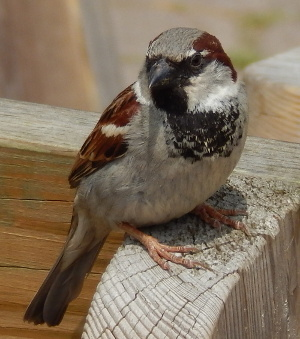
\includegraphics{images/sparrow.jpg}
\caption{\emph{Passer domesticus}}
\end{figure}

I performed an independent two-sample student's t-test on sparrow total
body length to test whether or not sparrows that died in the 1898 storm
were larger than sparrows that survived. I assume that both groups of
sparrows (dead and living) have equal variances, so the test statistic
\(t\) is calculated as follows,

\[t = \frac{\bar{X}_{1} - \bar{X}_{2}} {s_{p} \times \sqrt{\frac{1}{n_{1}} + \frac{1}{n_{2}}}}.\]

In the above, \(\bar{X}_{1}\) and \(\bar{X}_{2}\) are the mean of the
samples of sparrows that died and lived, respectively. Similarly,
\(n_{1}\) and \(n_{2}\) are the sample sizes of sparrows that died and
lived, and \(s_{p}\) is the pooled sample mean, which is calculated as
follows,

\[s_{p} = \sqrt{\frac{s^{2}_{X_{1}} + s^{2}_{X_{2}}}{2}}.\]

In the above, the \(s^{2}_{X_{1}}\) and \(s^{2}_{X_{2}}\) are the sample
standard deviations for sparrows that died and lived, respectively. I
conducted the two sample t-test using the \texttt{t.test} function in R
(\protect\hyperlink{ref-R2018}{R Core Team 2018}).

\hypertarget{results}{%
\section{Results}\label{results}}

\texttt{\{r,\ echo\ =\ FALSE,\ eval\ =\ TRUE\}\ dat\ \ \textless{}-\ read.csv(file\ =\ "data/Bumpus\_data.csv");\ res\ \ \textless{}-\ t.test(formula\ =\ dat\$totlen\ \textasciitilde{}\ dat\$surv,\ alternative\ =\ "less",\ \ \ \ \ \ \ \ \ \ \ \ \ \ \ \ \ var.equal\ =\ TRUE);\ \#\ Two\ sample\ t-test\ results\ tval\ \textless{}-\ as.numeric(res\$statistic);\ \#\ Get\ the\ t-test\ statistic\ pval\ \textless{}-\ res\$p.value;\ \#\ Get\ the\ p\ value\ from\ the\ t-test\ results\ live\ \textless{}-\ as.numeric(res\$estimate{[}1{]});\ \#\ Get\ mean\ length\ of\ living\ sparrows\ dead\ \textless{}-\ as.numeric(res\$estimate{[}2{]});\ \#\ Get\ mean\ length\ of\ dying\ sparrows}

Bumpus' data included \texttt{r\ sum(dat\$surv\ ==\ "alive")} sparrows
that lived and \texttt{r\ sum(dat\$surv\ ==\ "dead")} sparrows that
died. The mean total length of living sparrows was
\texttt{r\ round(live,\ digits\ =\ 2)} mm, and the mean total length of
dead sparrows was \texttt{r\ round(dead,\ digits\ =\ 2)} mm. The two
sample t-test revealed a t-statistic of
\texttt{r\ round(tval,\ digits\ =\ 2)}, which corresponds to a p-value
of \(P =\) \texttt{r\ round(pval,\ digits\ =\ 5)}.

\texttt{\{r,\ echo\ =\ FALSE,\ eval\ =\ TRUE\}\ total\_len\_alive\ \textless{}-\ dat\$totlen{[}dat\$surv\ ==\ "alive"{]};\ total\_len\_dead\ \ \textless{}-\ dat\$totlen{[}dat\$surv\ ==\ "dead"{]};\ summary\_alive\ \ \ \textless{}-\ summary(total\_len\_alive);\ summary\_dead\ \ \ \ \textless{}-\ summary(total\_len\_dead);}

Figure 2 shows the difference between total length in sparrows that
survived versus sparrows that died. Overall, dead sparrows were
\texttt{r\ round(dead\ -\ live,\ digits\ =\ 2)} mm longer than living
sparrows, and ranged between
\texttt{r\ as.numeric(summary\_dead{[}1{]})} and
\texttt{r\ as.numeric(summary\_dead{[}5{]})} mm. Living sparrows ranged
between \texttt{r\ as.numeric(summary\_alive{[}1{]})} and
\texttt{r\ as.numeric(summary\_alive{[}5{]})} mm (Figure 2).

\texttt{\{r,\ echo\ =\ FALSE,\ eval\ =\ TRUE,\ fig.width\ =\ 5,\ fig.height\ =\ 5,\ fig.cap\ =\ "Box\ plot\ of\ the\ total\ lengths\ of\ live\ and\ dead\ sparrows\ following\ a\ snowstorm\ in\ Providence,\ RI,\ as\ originally\ collected\ by\ Hermon\ Bumpus.\ The\ central\ horizontal\ line\ shows\ median\ values.\ Boxes\ and\ whiskers\ show\ inter-quartile\ ranges\ and\ extreme\ values,\ respectively."\}\ par(mar\ =\ c(5,\ 5,\ 1,\ 1));\ plot(x\ =\ as.factor(dat\$surv),\ y\ =\ dat\$totlen,\ cex.axis\ =\ 1.5,\ lwd\ =\ 2,\ \ \ \ \ \ ylab\ =\ "Total\ Sparrow\ Length\ (mm)",\ cex.lab\ =\ 1.5,\ \ \ \ \ \ \ xlab\ =\ "Sparrow\ status");}

\hypertarget{discussion}{%
\section{Discussion}\label{discussion}}

I have analysed data collected by Herman Bumpus
(\protect\hyperlink{ref-Bumpus1898}{Bumpus 1898}) on the relationship
between sparrow (\emph{Passer domesticus}) total length and surival
following an unusually severe storm. I found that sparrows that died in
the storm were longer than sparrows that survived, which suggests that
higher sparrow body length decreased survival. Of course, it is not
possible to definitively conclude a causal relationship between any
aspect of body size and sparrow survival , and even the available data
collected by Bumpus would permit a more thoughtful analysis than that
conducted in this study (see \protect\hyperlink{appendix}{Appendix Table
1}).

Overall, this document demonstrates how high quality, professional
looking documents can be written using Rmarkdown. The
\href{https://github.com/StirlingCodingClub/Manuscripts_in_Rmarkdown/blob/master/ms.Rmd}{underlying
code} for this manuscript is publicly available, along with
\href{https://stirlingcodingclub.github.io/Manuscripts_in_Rmarkdown/Rmarkdown_notes.html}{accompanying
notes} to understand how it was written. By using Rmarkdown to write
manuscripts, authors can more easily use version control (e.g., git)
throughout the writing process. The ability to easily integrate
citations though BibTeX, LaTeX tools, and dynamic R code can also make
writing much more efficient and more enjoyable. Further, obtaining the
benefits of using Rmarkdown does not need to come with the cost of
isolating colleagues who prefer to work with Word or LaTeX because
Rmarkdown can easily be converted to these formats (in the case of Word,
with the push of a button). By learning all of the tools used in this
manuscript, readers should have all of the necessary knowledge to get
started writing and collaborating in Rmarkdown.

\hypertarget{references}{%
\section{References}\label{references}}

\hypertarget{refs}{}
\begin{CSLReferences}{1}{0}
\leavevmode\vadjust pre{\hypertarget{ref-Bumpus1898}{}}%
Bumpus, H. C. 1898. {Eleventh lecture. The elimination of the unfit as
illustrated by the introduced sparrow, {\emph{Passer domesticus}}. (A
fourth contribution to the study of variation.)}. Biological Lectures:
Woods Hole Marine Biological Laboratory 209--225.

\leavevmode\vadjust pre{\hypertarget{ref-Darwin1859}{}}%
Darwin, C. 1859. {The Origin of Species}. Penguin, New York.

\leavevmode\vadjust pre{\hypertarget{ref-Johnston1972}{}}%
Johnston, R. F., D. M. Niles, and S. A. Rohwer. 1972. {Hermon Bumpus and
natural selection in the House Sparrow {\emph{Passer domesticus}} }.
Evolution 26:20--31.

\leavevmode\vadjust pre{\hypertarget{ref-R2018}{}}%
R Core Team. 2018. \href{https://www.R-project.org/}{R: A language and
environment for statistical computing}. R Foundation for Statistical
Computing, Vienna, Austria.

\end{CSLReferences}

\hypertarget{appendix-table-1}{%
\section{Appendix Table 1}\label{appendix-table-1}}

An example table is shown below, which includes all of the variables
collected by Bumpus (\protect\hyperlink{ref-Bumpus1898}{1898}) for the
first 10 measured sparrows. The full data set can be found online in
\href{https://github.com/StirlingCodingClub/Manuscripts_in_Rmarkdown/blob/master/data/Bumpus_data.csv}{GitHub}.

\texttt{\{r,\ echo\ =\ FALSE\}\ library(knitr);\ kable(x\ =\ dat{[}1:10,{]},\ caption\ =\ "First\ ten\ rows\ of\ the\ original\ data\ set\ collected\ by\ Hermon\ Bumpus");}

\end{document}
